
% JuliaCon proceedings template
\documentclass{juliacon}
\setcounter{page}{1}
\usepackage{amsmath,booktabs,mathtools,amssymb}
\newcommand{\term}[1]{\emph{#1}}
%
\hypersetup{colorlinks=true}
%
\begin{document}

% **************GENERATED FILE, DO NOT EDIT**************

\title{My JuliaCon proceeding}

\author[1]{1st author}
\author[1, 2]{2nd author}
\author[2]{3rd author}
\affil[1]{University}
\affil[2]{National Lab}

\keywords{Julia, Optimization, Game theory, Compiler}

\hypersetup{
pdftitle = {My JuliaCon proceeding},
pdfsubject = {JuliaCon 2022 Proceedings},
pdfauthor = {1st author, 2nd author, 3rd author},
pdfkeywords = {Julia, Optimization, Game theory, Compiler},
}


% TODO : How to specify an email-address?
\maketitle

\begin{abstract}
    \href{https://juliamanifolds.github.io/LieGroups.jl/stable/}{\texttt{LieGroups.jl}} is a
    Julia package that provides on the one hand an interface to define Lie groups as well as the corresponding Lie algebra and Lie group actions. On the other hand, it offers a well-documented, performant, and well-tested library of existing Lie groups, their Algebra and corresponding group actions.

    This paper presents the main features of the interfaces and how that is integrated within
    the \verb|JuliaManifolds| ecosystem. We further present an overview on existing Lie groups
    implemented in \verb|LieGroups.jl| as well as how to get started to use the package in practice.
\end{abstract}
%
\section{Introduction}%
\label{sec:Introduction}
%
In many situations, one encounters data that does not reside in a vector space.
We can hence not used standard linear algebra tools to work with such data.
For example in robotics, the configuration space of a rigid body in three-dimensional
space is given by the special Euclidean group \(\mathrm{SE}(3)\),
consisting of all translations and rotations.
A subset of these is the space of rotations, given by the special orthogonal group \(\mathrm{SO}(3)\),
or more generally \(\mathrm{SO}(n)\) in \(n\)-dimensional space.

These spaces are examples of Lie groups, formally defined as a smooth manifold equipped with a group structure.
They have applications e.g.\ in physics, robotics, stochastic processes, information geometry, see e.g.~\cite{Chirikjian:2009,Chirikjian:2012},
but are also interesting from their mathematical viewpoint~\cite{HilgertNeeb:2012}
and their numerical aspects, e.g.\ when solving differential equations on Lie groups~\cite{Munthe-Kaas:1998}.

The package~\href{https://juliamanifolds.github.io/LieGroups.jl/stable/}{\texttt{LieGroups.jl}}\footnote{%
Available at~\href{https://juliamanifolds.github.io/LieGroups.jl/stable/}{juliamanifolds.github.io/LieGroups.jl/stable/},
see also the zenodo archive~\cite{LieGroups.jl}.%
}
provides an easy access to both defining and using Lie groups within
the Julia programming language~\cite{bezanson2017julia} by defining an interface of Lie groups, as well as implementing a library of Lie groups, that can directly be used.

This paper provides an overview of the main features of \verb|LieGroups.jl|.
After introducing the necessary mathematical background and notation in Section~\ref{sec:Notation},
we present the interface in Section~\ref{sec:Interface}, split into the Lie group, the Lie algebra, and group actions.
In Section~\ref{sec:LieGroups}, we present an overview of currently implemented Lie groups.
Finally, in Section~\ref{sec:Example}, we demonstrate how to get started and use \verb|LieGroups.jl|.

\section{Mathematical Background}%
\label{sec:Notation}

\begin{figure}
    \centering
    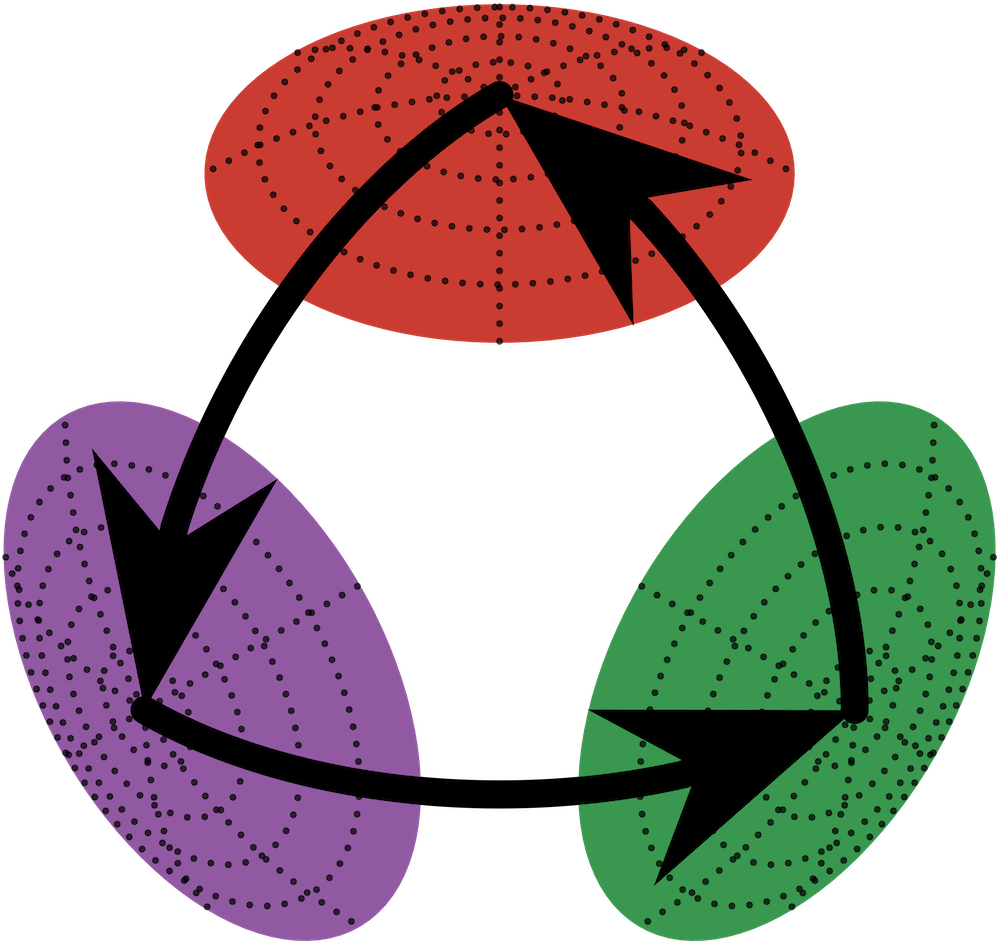
\includegraphics[width=0.1875\textwidth]{logo.png}
    \caption*{\ \\[-.5\baselineskip]Logo of \texttt{LieGroups.jl}.}%
    \label{fig:liegroups_logo}
\end{figure}

The following notation and definitions follow the text book~\cite{HilgertNeeb:2012},
for more details on Riemannian manifolds, see also~\cite{DoCarmo:1992}.

We denote a Lie group by \(\mathcal{G} = (\mathcal{M}, \cdot)\) where \(\mathcal{M}\) is a smooth manifold and \(\cdot\) is the group operation.
A smooth manifold \(\mathcal{M}\) is a topological space that is locally isomorphic to an Euclidean space \(\mathbb{R}^n\) for some \(n \in \mathbb{N}\), but globally may have a different topology.
We call \(n\) the dimension of the manifold \(\mathcal{M}\), denoted by \(\dim(\mathcal{M}) = n\).
As an example, take the \(2\)-dimensional sphere \(\mathbb{S}^2 = \{x \in \mathbb{R}^3 \mid \lVert x\rVert = 1\}\),
which locally looks like \(\mathbb{R}^2\), think of charts in an atlas, but globally it is not.
Finally we denote the tangent space at a point \(p \in \mathcal{M}\) by \(T_p\mathcal{M}\). This can be thought of as all “velocities” (direction and speed) in which a curve can “pass through” a point. Formally it is set the equivalence classes of derivatives of smooth curves. Each tangent space $T_p\mathcal M$ is a $n$-dimensional vector space and we call the disjoint union of all tangent spaces $T\mathcal M = \dot\bigsqcup_{p \in \mathcal M} T_p\mathcal M$ the \term{tangent bundle} of $\mathcal M$.

As a group operation \(\cdot\colon\mathcal{G} \times \mathcal{G} \to \mathcal{G}\) has to satisfy the group axioms associativity, existence of an identity element \(e \in \mathcal{G}\), and existence of inverses \(x^{-1} \in \mathcal{G}\) for all \(x \in \mathcal{G}\). Furthermore the group operation \(\cdot\) (on \( \mathcal{G}\times\mathcal{G} \)) and the inversion map \(\iota\colon\mathcal{G} \to \mathcal{G}, x \mapsto x^{-1}\) have to be smooth maps.
As an example, consider the special orthogonal group \(\mathrm{SO}(n)\), consisting of all \(n \times n\) orthogonal matrices, with determinant \(1\), i.e.\ for \(p\in \mathrm{SO}(n)\), we have \(p^{\mathrm{T}} p = I\) and \(\det(p) = 1\) together with the group operation \(\cdot\) given by matrix multiplication.
For $n=2$ these are rotations in the plane, hence each operation can be identified with an angle $\alpha \in [-\pi, \pi)$, or in other words the circle. % chktex 9ok
The identity element is given by the identity matrix \(I\) (or the angle $\alpha=0$) and the inverse of a rotation matrix is given by its transpose (or an angle $-\alpha$).

The tangent space at the identity element \(e \in \mathcal{G}\), denoted by \(\mathfrak{g} = T_e\mathcal{G}\), plays a special role and is called the \term{Lie algebra} of the Lie group \(\mathcal{G}\).
The reason is that to represent arbitrary tangent vectors $X \in T_g\mathcal{G}$ at a point $g \in \mathcal{G}$, since we can use the group operation: we denote by $\lambda_g(h) = g \cdot h$ the left multiplication with $g, h \in \mathcal{G}$.
Then, using the differential (or pushforward) $D\lambda_g(h)\colon T_g\mathcal G \to T_h\mathcal G$, we can generate a so-called \term{left-invariant vector field} $\mathcal X(g) \coloneqq D\lambda_g(e)[X]$ which is uniquely determined by the choice of $X \in \mathfrak{g}$.
Hence we can identify tangent vectors $\mathcal X(g) \in T_g\mathcal G$ at arbitrary points $g \in \mathcal G$ with $X$ from the Lie algebra $\mathfrak{g}$.

Finally, a \term{group action} of a Lie group \(\mathcal{G}\) on a smooth manifold \(\mathcal{M}\) is a smooth map \(\rho\colon \mathcal{G} \times \mathcal{M} \to \mathcal{M}\) such that for all \(g, h \in \mathcal{G}\) and \(p \in \mathcal{M}\) it holds that \(\rho(e, p) = p\) and \(\rho(g, \rho(h, p)) = \rho(g \cdot h, p)\).
Informally a group action describes how elements of the Lie group \(\mathcal{G}\) “act on” points on the manifold \(\mathcal{M}\). As an example, think of the special orthogonal group \(\mathrm{SO}(3)\) acting on points on Euclidean space $\mathbb{R}^3$ “moving” them somewhere by rotating them around the origin. The same action can also be applied to points from the sphere \(\mathbb{S}^2\).

\section{The interface}\label{sec:Interface}

Since a Lie group \(\mathcal{G}\) consists of two main components, the smooth manifold \(\mathcal{M}\) and the group operation \(\cdot\), we can reuse existing functionality from the existing interface for manifolds provided by \verb|ManifoldsBase.jl|, and later concrete manifolds provided by \verb|Manifolds.jl|~\cite{AxenBaranBergmannRzecki:2023}.
This is done in a transparent way, i.e.\ the \verb|AbstractLieGroup| itself is a subtype of \verb|AbstractManifold| from \verb|ManifoldsBase.jl| and can hence also be used in all existing places, as for example optimization on manifolds provided by \verb|Manopt.jl|~\cite{Bergmann:2022}.

\subsection{Lie groups}
{\color{red} TODO 1-1.5 pages on the interfaces and main functions provided for Lie groups and group operations, Lie algebra, and group actions. Maybe take over some story parts from the talk.}

\cite{HilgertNeeb:2012}

\subsection{Lie algebras}
\subsection{Group actions}

\section{Implemented Lie groups}\label{sec:LieGroups}
\begin{table}[tbp]
    \centering
    \caption{Implemented Lie groups in \texttt{LieGroups.jl} as of version 0.1.6}
    \begin{tabular}{@{}lll@{}}
        \toprule
        \textbf{Group} & \textbf{Symbol} & comment/code\\
        \midrule
        \verb|CircleGroup()| & \(\mathbb{S}^1\) & 3 representations \\
        \verb|GeneralLinearGroup(n, F)| & \(\mathrm{GL}(n, \mathbb{F})\) & $\mathbb{F} \in \{\mathbb{R}, \mathbb{C}\}$\\
        \verb|HeisenbergGroup(n)| & \(\mathrm{H}(n)\)\\
        \verb|OrthogonalGroup(n)| & \(\mathrm{O}(n)\) &\\
        \midrule
        \verb|PowerLieGroup(G, n)| & \(\mathcal G^n\) & \verb|G^n|\\
        \verb|ProductLieGroup(G1, G2,...)| & \(\mathcal G_1 \times \mathcal G_2 \times \ldots\) & \verb|G1| $\times$ \verb|G2| $\times$ \ldots\\
        Semidirect product group & \(\mathcal G_1 \ltimes \mathcal G_2\) & \verb|G1| $\ltimes$ \verb|G2|\\
                                 & \(\mathcal G_1 \rtimes \mathcal G_2\) & \verb|G1| $\rtimes$ \verb|G2|\\
        \midrule
        \verb|SpecialEuclideanGroup(n)| & \(\mathrm{SE}(n)\) & \\
        \verb|SpecialGalileanGroup(n)| & \(\mathrm{SGal}(n)\) &  \\
        \verb|SpecialLinearGroup(n, F)| & \(\mathrm{SL}(n, \mathbb{F})\) & $\mathbb{F} \in \{\mathbb{R}, \mathbb{C}\}$\\
        \verb|SpecialOrthogonalGroup(n)| & \(\mathrm{SO}(n)\) &  \\
        \verb|SpecialUnitaryGroup(n)| & \(\mathrm{SU}(n)\) & \\
        \midrule
        \verb|SymplecticGroup(n)| & \(\mathrm{Sp}(2n)\) & \\
        \verb|TranslationGroup(n; field=|$\mathbb{F}$\verb|)| & \(\mathbb{F}^n\) & $\mathbb{F} \in \{\mathbb{R}, \mathbb{C}, \mathbb{H}\}$\\
        \verb|UnitaryGroup(n)| & \(\mathrm{U}(n)\) & \\
        \bottomrule
    \end{tabular}
\end{table}

\section{An example how to use {\texttt{LieGroups.jl}}}\label{sec:Example}
% **************GENERATED FILE, DO NOT EDIT**************

\bibliographystyle{juliacon}
\bibliography{ref.bib}

\end{document}
%
% ------------------------------------------------------------------------------------------
%


\subsection{Writing Julia code}

A special environment is already defined for Julia code,
built on top of \textit{listings} and \textit{jlcode}.

\begin{verbatim}
\begin{lstlisting}[
    language = Julia,
    numbers=left,
    label={lst:exmplg},
    caption={Example Code Block.}
]
using Plots

x = -3.0:0.01:3.0
y = rand(length(x))
plot(x, y)
\end{lstlisting}
\end{verbatim}
\begin{lstlisting}[
    language = Julia,
    numbers=left,
    label={lst:exmplg},
    caption={Example Code Block.}
]
using Plots

x = -3.0:0.01:3.0
y = rand(length(x))
plot(x, y)
\end{lstlisting}

\subsection{Balancing column at last page}
\label{subsub:Balance}
For balancing the both column length at last page use :
\begin{verbatim}
\vadjust{\vfill\pagebreak}
\end{verbatim}

%\vadjust{\vfill\pagebreak}

at appropriate place in your \TeX{} file or in bibliography file.
